\chapter{Metodologia}
O software tem que demostrar que serve para a situação proposta, com isso, diferentes rotas em situações onde é possível encontrar o caminho, ou não, foram criadas de forma a testar o software e evitar possíveis erros ou falsos positivos.
Utilizando a API do Google Maps como fonte de dados, informações reais de distância, tempo médio e localização são utilizadas para uma simulação mais próxima de uma situação real.

Por se tratar de entregas de pequenos porte, os testes foram criados com coordenadas a nível de cidade, São Paulo é a cidade para os testes, por se tratar de uma cidade com um alto índice de transito segundo o TomTom Traffic Index \cite{TomTom}, a menor rota pode não será a melhor escolha para aquele horário do dia.

Todos os entregadores saem de uma única origem, antes de começar a entrega, é calculada uma rota geral, e ela é dividida de forma a entregar rotas possível para cada entregar, se o limite de entregados for ultrapassado, um avisa será emitido recomendando que deixe para o próximo dia as entregas mais distantes.

Cada destino tem um período permitido para entrega, e cada entrega demora no máximo 5 minutos para ser descarregada. Depois que uma entrega é feita, o software recalcula o próximo destino com base no transito atual e o período para entregar.
Se caso não é mais possível entregar no horário por causa do transito piorou, um alerta será emitido. Depois que o entregador terminou todas suas entregas, o software continua auxiliando os outros entregadores, até concluir todas as entregas.

O fluxograma a baixo demostra o funcionamento do software.

\begin{minipage}{\linewidth}
	\makebox[\linewidth]{
		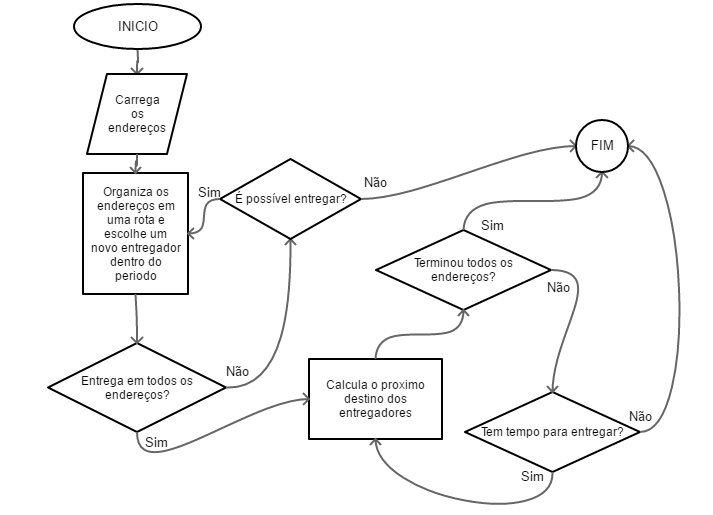
\includegraphics[keepaspectratio=true,scale=0.5]{ibagens/Fluxograma.png}}
	\captionof{figure}{Fluxograma macro do funcionamento do software.  }
	\label{fig:FluxoSoftare}
\end{minipage}

Nos testes foram definidas rotas pré-definidas para possíveis problemas, ignorando o transito atual. por que o transito altera dependendo das condições do clima ou horário do dia. Então utilizando o Google Maps, um cache inicial foi preparado e o software utiliza simulando uma buscar ao Google Maps, com isso, a informação é obtida mais rapidamente e sempre fixa para garantir a resposta pre-determinada do teste.

\chapter{Implementação}
 
Nesse capitulo será apresentado mais aprofundadamente as ferramentas e métodos que foram utilizados para a implementação do algoritmo genético para busca de rota com janela de tempo.
 
\section{O Projeto}
O software é separado em três projetos, todos utilizando .Net Core 2.0 com a linguagem C\# no Visual Studio 2017 para plataforma Windows ou \**nix.
O \textbf{PathFinder.Routes} nesse projeto estão os algoritmos de comunicação com o Google Maps e organização de rotas. 
O \textbf{PathFinder.GeneticAlgorithm} nesse projeto estão as implementações para a utilização do algoritmo genético.
O \textbf{PathFinder} projeto principal para inicialização do software e utiliza os dois outros projetos em sua implementação.

\section{Organização}
Os projetos são organizados utilizando o padrão do visual studio chamado de Solution.

\subsection{PathFinder}
Projeto de inicialização no modo console, todo progresso do software é exibido em texto.

\textbf{Program:} Implementação das união de todas as classes, executa a separação dos entregadores.

\textbf{Entregador:} Informação individual, armazena a rota completa do entregar e o genoma representante.

\textbf{TimeMeasure:} Configuração de registro/exibição do tempo de processamento.
\subsection{PathFinder.Routes}

\subsection{PathFinder.GeneticAlgorithm}


\section{Funcionalidades}

\section{Testes}